\section{Evaluation}
\begin{frame}
  % \centering
  \huge
  \red{Evaluation}
\end{frame}

\begin{frame}
  \frametitle{Usability}
  \centering
  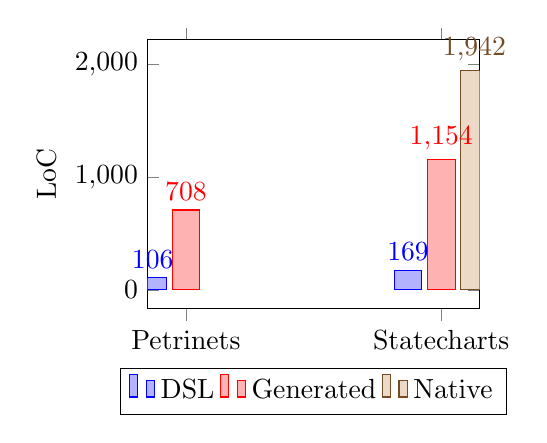
\begin{tikzpicture}
    \begin{axis}[
      height=5cm,
        ybar,
        enlargelimits=0.15,
        legend style={at={(0.5,-.22)},
          anchor=north,legend columns=-1},
        ylabel={LoC},
        symbolic x coords={Petrinets,Statecharts},
        xtick=data,
        nodes near coords,
        nodes near coords align={vertical},
        ]
    \addplot coordinates {(Petrinets,106) (Statecharts,169)};
    \addplot coordinates {(Petrinets,708) (Statecharts,1154)};
    \addplot coordinates {(Statecharts,1942)};
    \legend{DSL,Generated,Native}
    \end{axis}
    \end{tikzpicture}
\end{frame}

\begin{frame}
  \frametitle{Performance}\centering
  \begin{tikzpicture}
    \begin{axis}[
        width=.8\linewidth,
        height=5cm,
        ylabel={Processing time in ms},
        xlabel={Number of States},
        legend style={at={(.1,-.2)},
          anchor=north},
        xtick={1,2,3,4,5,6,7,8,9,10,11},
        xticklabels={9,16,25,36,49,64,81,100,121,144,169}
      ]
      \addplot table [x=a, y=b, col sep=comma] {generatedimpl.csv};
      \addlegendentry{generated}
      \addplot table [x=a, y=b, col sep=comma] {nativeimpl.csv};
      \addlegendentry{native}
    \end{axis}
  \end{tikzpicture}
\end{frame}

\begin{frame}
  % \frametitle{Plugins}
  \centering
  \huge
  \red{Plugins}
\end{frame}